
In next chapters, more advanced control techniques will be treated. All of them are based on the state-space realization of the system, so a reconstruction of the state is needed since some signals are not available because too noisy to be used (i.e. motor and masses speed, derived by potentiometer and encorders position readings).

\section{State observer}

The gray-box models, identified in \cref{sec:gray_b_id}, are sufficiently precise to be used for observers design. The state reconstruction is performed by using motor and masses position signals; poles of the closed-loop observer are placed in a prescribed position: they must be sufficiently far from the imaginary axis so that asymptotic stability is ensured~(even considering poles uncertainty) and, moreover, time settlement of the observer is satisfactorily low.

\paragraph{\acrshort{1-dof} system}

In order to construct the observer, matrices A and C are needed~(where C matrix identifies the available signals, paying attention to those sign). In case of \acrshort{1-dof} system:

\begin{equation}
	A = 
	\begin{bmatrix}
		0 &1 & 0 & 0 \\
		-\frac{K_{s_1}}{J_m} & -\frac{B_m}{J_m}-\frac{\eta_m \eta_g k_t k_m {K_g}^2}{R_m J_m}  & \frac{K_{s_1}}{J_m} & 0 \\
		0 & 0 & 0 & 1 \\
		\frac{K_{s_1}}{J_1} & 0 & -\frac{K_{s_1}}{J_1} & -\frac{B_1}{J_1}
	\end{bmatrix}
	\qquad
	C =
	\begin{bmatrix}
		1 & 0 & 0 & 0 \\
		0 & 0 & -1 & 0
	\end{bmatrix}
\label{eqn:1dof_mat_obs}
\end{equation}

Closed-loop poles can be automatically placed in prescribed positions thanks to the MATLAB function~\textit{place}\footnote{This function requires to locate poles in different positions. To place poles in a unique position, it is sufficient to slightly move some of them.}.
The choice for poles frequency is~$400 \, rad/s$, meaning that the settling time of the observer is about 12.5 ms.

The estimated state dynamics, then, becomes
\begin{equation}
	\dot{\hat{x}}(t) = A\hat{x}(t) + Bu(t) + L [y(t) - C\hat{x}(t) - Du(t)] = (A-LC)\hat{x}(t) + (B-LD)u(t) + Ly(t)
	\label{eqn:est_state_dyn}
\end{equation}
and its estimation error dynamics is asymptotically stable, as pole placement prescribed:
\begin{equation}
	\dot{\hat{e}} (t) = (A-LC) \hat{e} (t)
\end{equation}

The necessary and sufficient condition to guarantee observer design and asymptotic stability is that pair~$(A,C)$ is observable. In this case, the rank of observability matrix is 4~(as the order of the system). \\

The initial position of the system, detected by the potentiometer, is subtracted to all position readings~(motor, first mass and, if connected, second mass); this causes a shift in state reconstruction that will never be recovered. Actually, this does not represent a problem since this kind of observer is only used for pole-placement controllers: as shown later, this will automatically bring the system to the correct reference, i.e.\ in the middle of potentiometer electrical range, thanks to an integral action.

In \cref{fig:observer_1dof}, a position control (performed by pole-placement, introduced in next chapter) is reported. It can be seen that the position of motor and first mass are shifted with respect to their measurements because of the initial position; however, position reconstructions perfectly superimpose measurements, as expected.\\
Concerning the speeds, mass velocity is a bit different from the measured one~(derived by the encoder), while motor speed is noisy because of potentiometer high variance; in any case, small differences on speed are not critical, since speed signals are not significantly weighted in next control techniques.

\paragraph{2-d.o.f. system}

Actually, the \acrshort{2-dof} observer structure is very similar to the previous one; matrices dimensions and available signals are different: in this case, in addition to potentiometer and first mass encoder, also the second mass position is available thanks to the last encoder. This means that matrix C has one more row:
\begin{equation}
	A = 
	\begin{bmatrix}
		0 &1 & 0 & 0 & 0 & 0 \\
		-\frac{K_{s_1}}{J_m} & -\frac{B_m}{J_m}-\frac{\eta_m \eta_g k_t k_m {K_g}^2}{R_m J_m}  & \frac{K_{s_1}}{J_m} & 0 & 0 & 0 \\
		0 & 0 & 0 & 1 & 0 & 0 \\
		\frac{K_{s_1}}{J_1} & 0 & -\frac{K_{s_1}+K_{s_2}}{J_1} & -\frac{B_1}{J_1} & \frac{K_{s_2}}{J_1} & 0 \\
		0 & 0 & 0 & 0 & 0 & 1 \\
		0 & 0 & \frac{K_{s_2}}{J_2} & 0 & -\frac{K_{s_2}}{J_2} & -\frac{B_2}{J_2}
	\end{bmatrix}
	C =
	\begin{bmatrix}
		1 & 0 & 0 & 0 & 0 & 0 \\
		0 & 0 & -1 & 0 & 0 & 0  \\
		0 & 0 & 0 & 0 & -1 & 0
	\end{bmatrix}
\label{eqn:2dof_mat_obs}
\end{equation}

This time, poles have been located in different positions: 2 of them in~$-300 \, rad/s$ and the other 4 in~$-400 \, rad/s$. Also in this case, $\mathit{O}$ matrix of the pair~$(A,C)$ is full rank. As in the~\acrshort{1-dof} case, a comparison between measured and reconstructed signals (figure~\ref{fig:observer_2dof}) shows that positions are very precisely estimated, while speeds are noisy and shifted in time.

\begin{figure*}
	\centering
	\begin{subfigure}{0.45\columnwidth}
		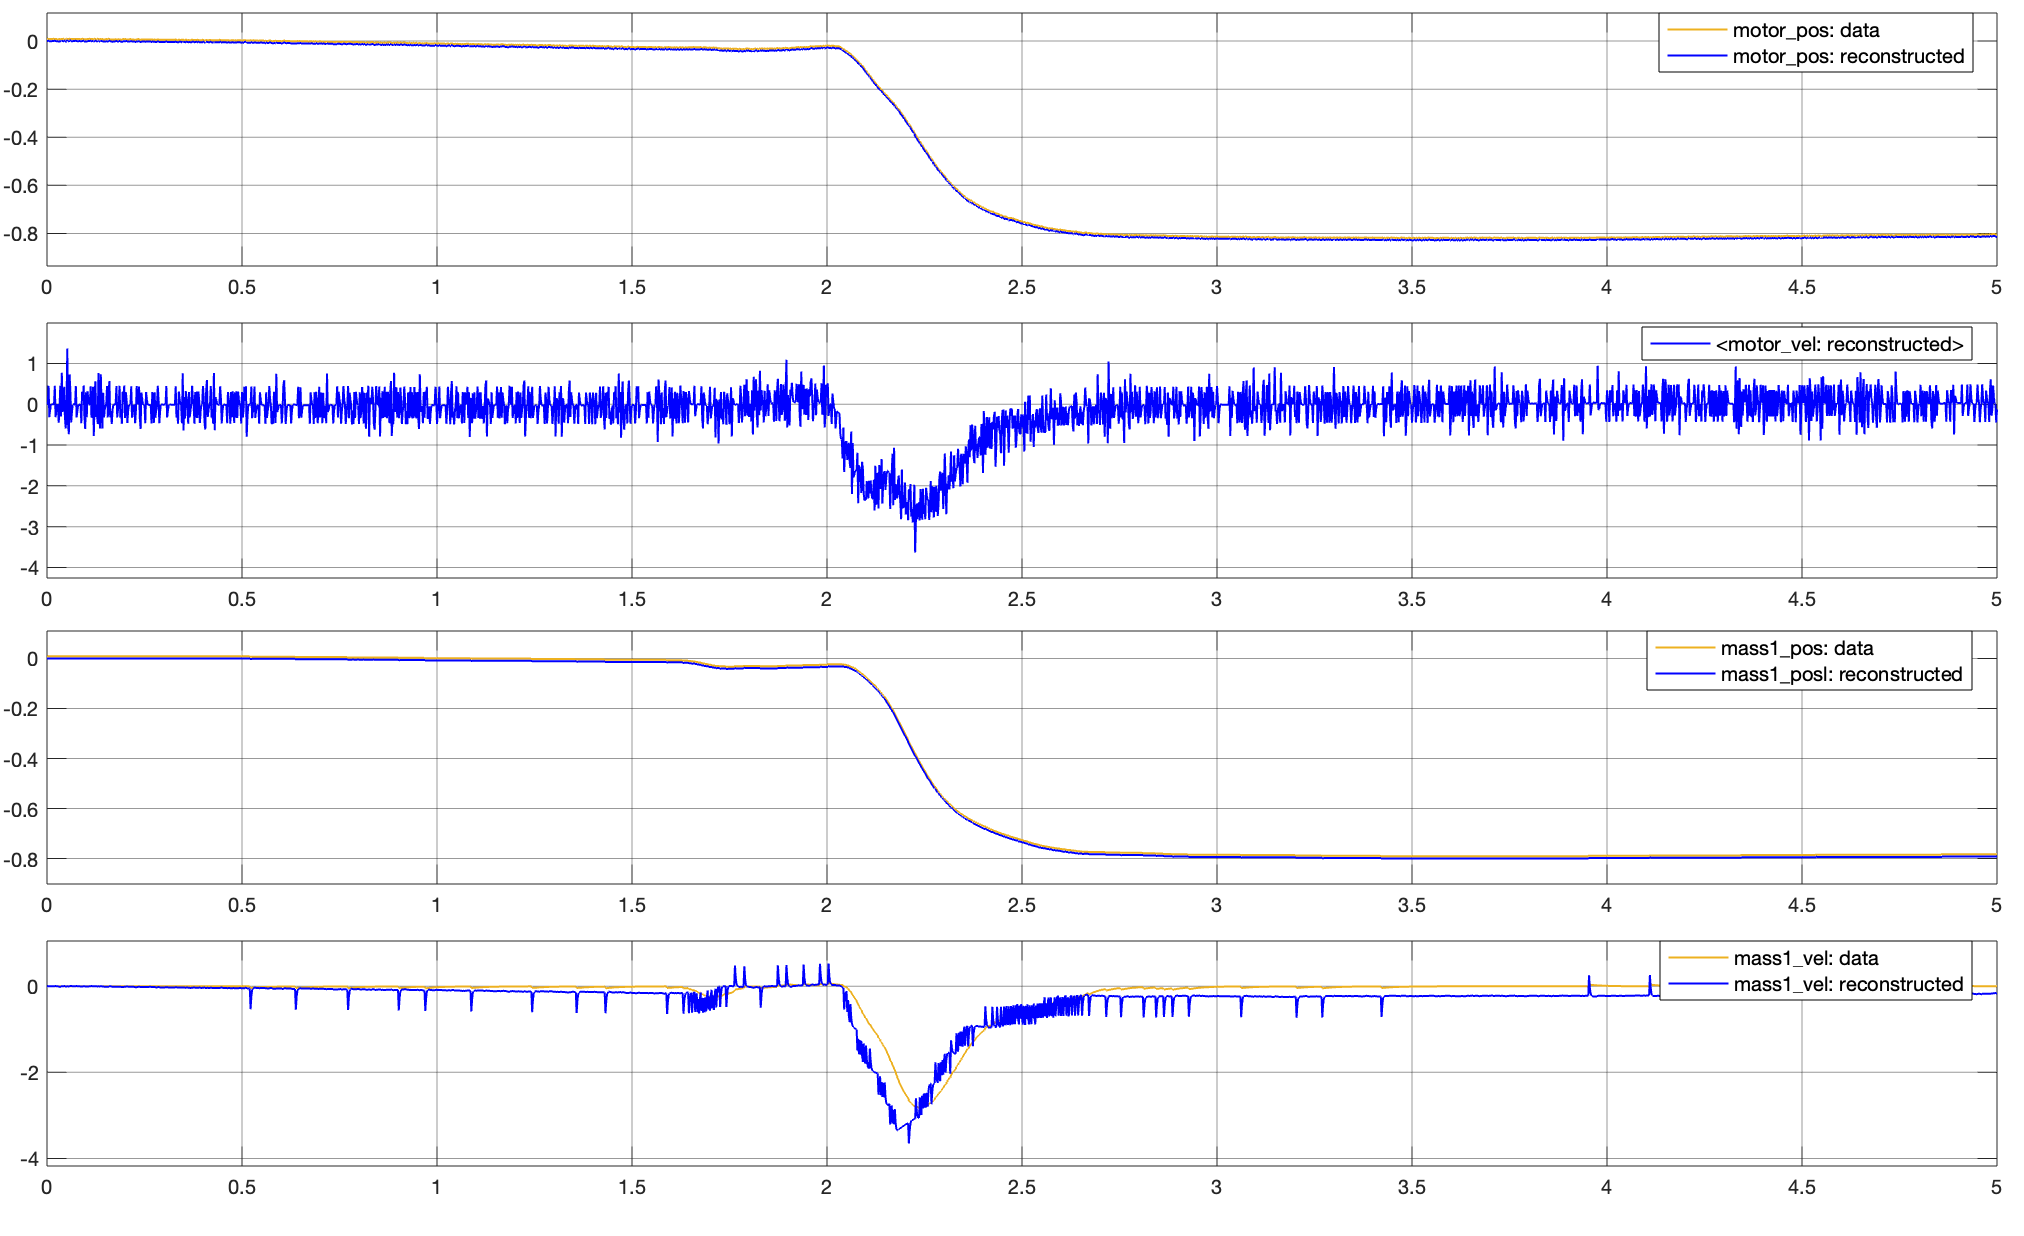
\includegraphics[width=\textwidth]{observer_1dof}
		\subcaption{\acrshort{1-dof} case}
		\label{fig:observer_1dof}
	\end{subfigure}
	\begin{subfigure}{0.45\columnwidth}
		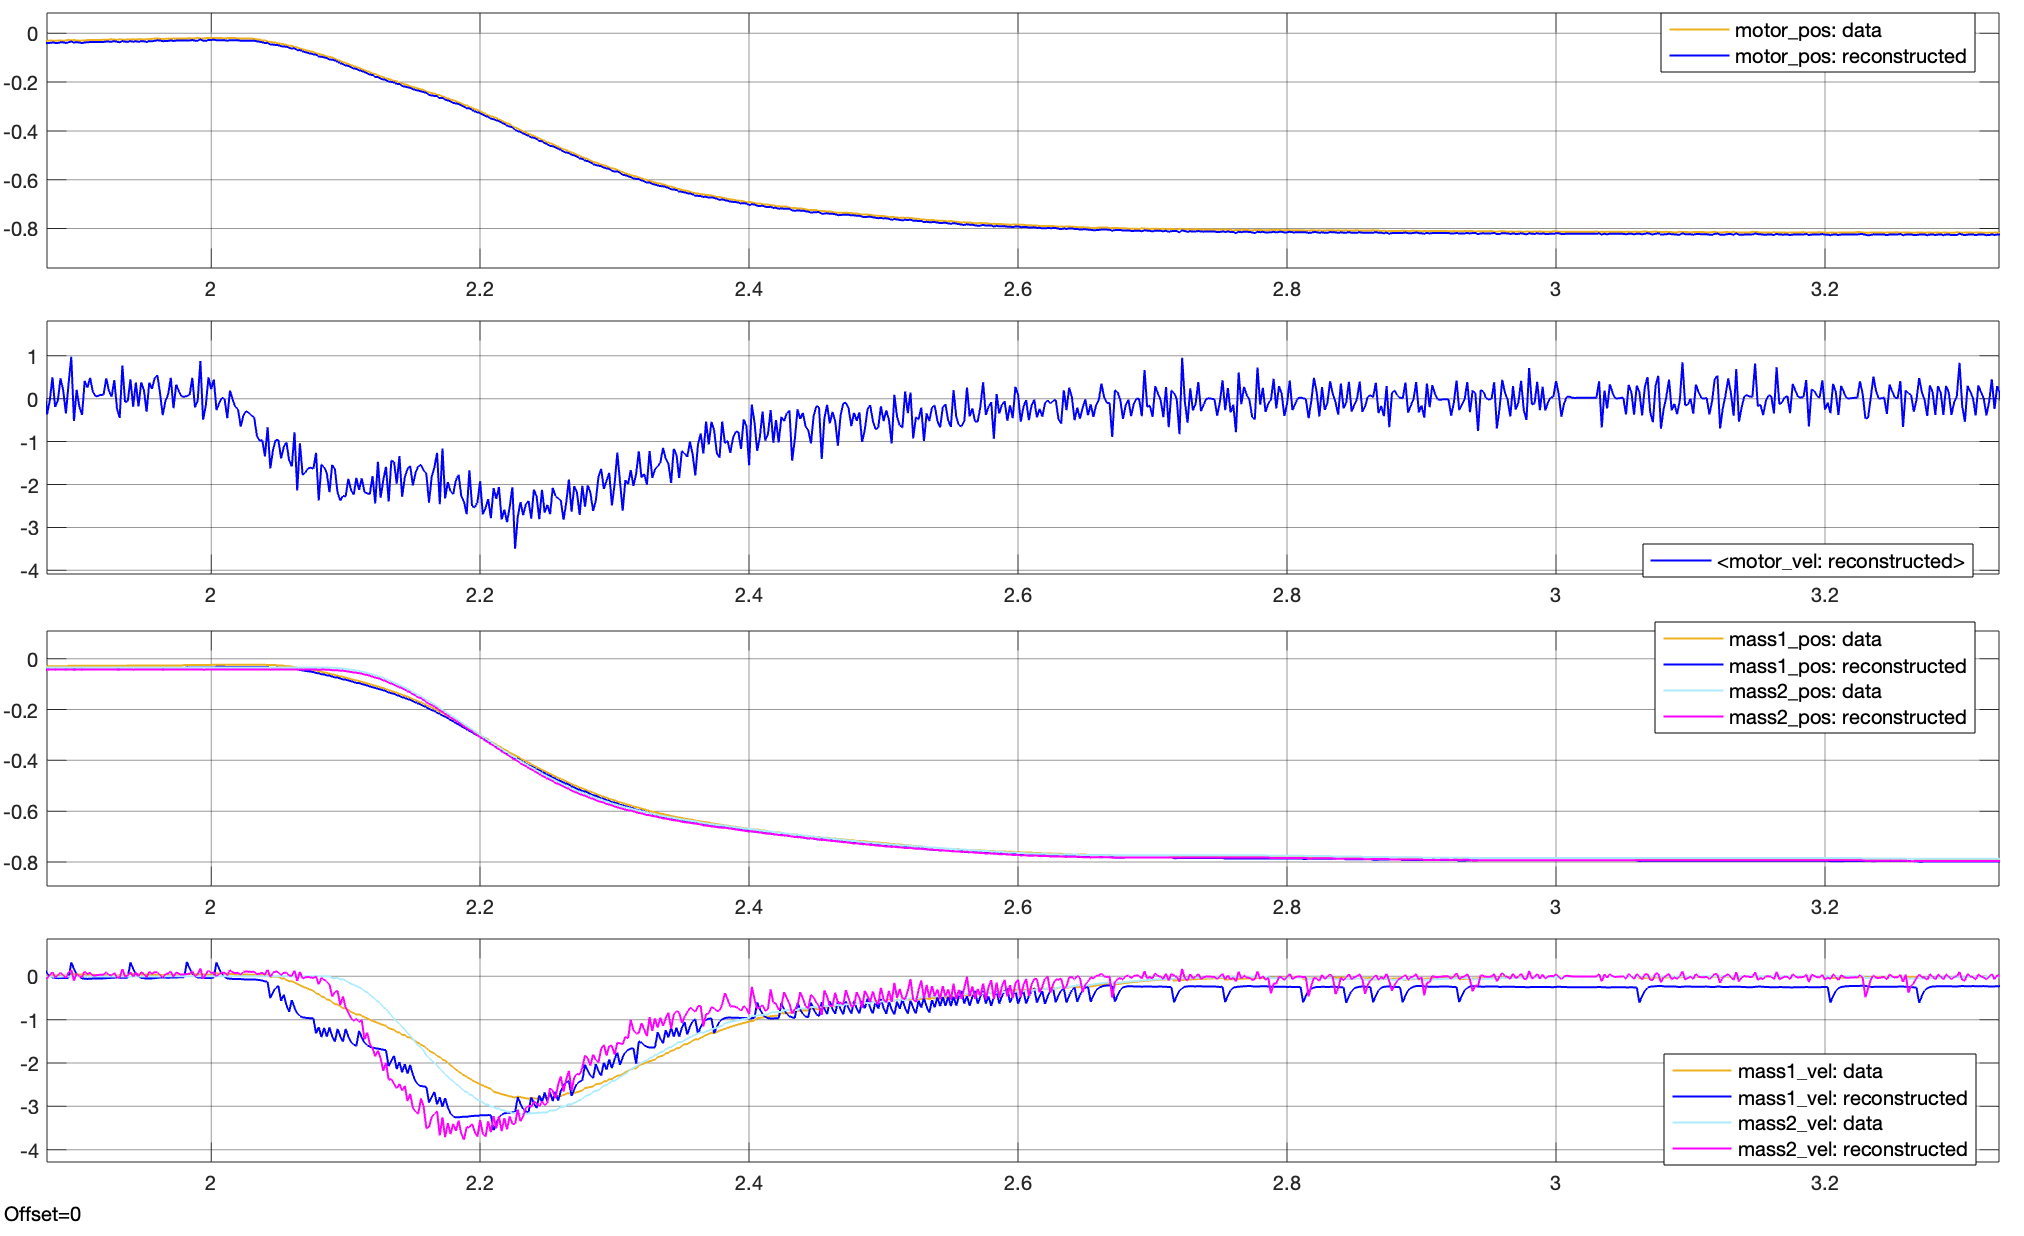
\includegraphics[width=\textwidth]{observer_2dof}
		\subcaption{\acrshort{2-dof} case}
		\label{fig:observer_2dof}
	\end{subfigure}
	\caption{Observer reconstruction compared to available measurements}
\end{figure*}

\section{Kalman filter}

The state reconstruction based on Luenberg observer works fine in abscence of any disturbance. Unfortunately, as mentioned in \cref{sec:sensors}, sensors produce signals at each sampling time that can be considered as stochastic variables. These variables have a variance that depends on the intrinsical characteristic of the sensors. The solution to represent this kind of behaviour, consist in separating the measurement signal $y(t)$ in a component deriving from the states, that can be considered the real value, and a component due to a white noise with a given covariance.  \\
With a mathematical description 

\begin{equation}
	\begin{cases}
		\dot x(t) =\ A x(t) + B u(t) +n_x(t) \\
		y(t) =\ C x(t) + D u(t) + n_y(t)
	\end{cases}
\end{equation}
where $n_x$ and $n_y$ are independent zero-mean white Gaussian processes having covariances
\begin{center}
	$E[n_x(t)n_x'(t)]=Q_x \delta(t-s)$  and $E[n_y(t)n_y'(t)]=Q_y \delta(t-s) $
\end{center}
for some $Q_x = Q_x' \geq 0$ and $Q_y = Q_y' > 0$, where $E[v]$ denotes the expected value of a random variable $v$.\\
The stationary version of the Kalman filtering problem can be posed as the task of generating a reconstruction $\hat x (t)$ of the state vector $x(t)$ using measurement $y(t)$ that minimize 
\begin{equation}
	\lim_{t \to \infty }E[ ||x(t) - \hat x(t) ||^2 ]
\end{equation}
which is the steady state variance of the reconstruction error $ x-\hat x$.\\
Although the original estimation problem didn't take in account any measured input $u$, in presence of it, it is possible to slightly modify the equations for the estimation. 
The estimated state dynamics is a stable and causal LTI system, with equation as \cref{eqn:est_state_dyn}. \\
The $L$ gain is the result of the filtering problem, for the generalized plant, without input $u$. \\
To obtain it, exogneous input $w$, that is any zero-mean unit-intensity white process such that
\begin{equation}
	\begin{bmatrix}
		n_x(t) \\
		n_y(t)
	\end{bmatrix} = 
	\begin{bmatrix}
		B_wB_w'& B_wD_w'\\
		D_wB_w' & D_wD_w'
	\end{bmatrix} w(t)
\end{equation}
is defined. \\
Under the assumption that noises $n_x$ and $n_y$ are uncorrelated, i.e. $B_wD_w' = 0$, the $L$ matrix is obtained solving a Riccati equation, involving also the other system matrices, that is
\begin{equation}
	Y = AYA' + B_wB_w' + (AYC'+B_wD_w')(CYC'+D_wD_w')^{-1}(CYA'+D_wB_w')
	\label{eqn:riccati_kf}
\end{equation}
where $Y = Y' \geq 0$.\\
Then, 
\begin{equation}
	L = (AYC'+B_wD_w')(CYC'+D_wD_w')^{-1}
	\label{eqn:kf_gain}
\end{equation}

\paragraph{Full sensors use}
Given the above definition of the problem, the 1-d.o.f. and the 2-d.o.f. systems generate similar solutions and make use of the same matrices as in \cref{eqn:1dof_mat_obs} and \cref{eqn:2dof_mat_obs}.
The $Q_y$ matrix is defined based on the variances computed at \cref{sec:sensors} and it is kept constant through all the development of this tool. 
On the other hand, matrix $Q_x$ doesn't depend directly on some physical properties and can be used to tune the filter. 
This means that by varying the parameters in this matrix, the solutions of the filtering problem change. \\
Moreover, this matrix can be considered as the uncertainty derived from the model identification process, i.e. since matrices $A$ and $B$ of the system have been computed by grey-box estimation (\cref{sec:gray_b_id}), they are naturally uncertain as they can't capture the real dynamic of the system that is much more complicated. \\
The obtained model can simulate much better the position of the masses then that of the motor shaft, this because during the identifcation process those measurements where taken with the encoder, that is much more accurate than the potentiometer. This translates in a higher value of the state variance for the shaft position then that of the masses. With a similar reasoning, speed states are more uncertain then position ones, as they are derived from them. Trying to balance the filter reliabilty (keeping $Q_x$ as high as possible) and filter settling time (keeping $Q_x$ as low as possible) these are the matrices that better suit the filtering problem.
\begin{equation}
	B_w = \begin{bmatrix}
		0.3e-4 & 0 & 0 & 0 & 0 & 0\\
		0 & 1e-2 & 0 & 0 & 0 & 0 \\
		0 & 0 & 1e-8 & 0 & 0 & 0  \\
		0 & 0 & 0 & 1e-4 & 0 & 0
	\end{bmatrix} \
	D_w = \begin{bmatrix}
		0 & 0 & 0 & 0 & 1e-6 & 0\\
		0 & 0 & 0 & 0 & 0 & 2e-8 
	\end{bmatrix} 
	\label{eqn:b_w_d_w}
\end{equation}
For the 2-d.o.f system the matrices have the same values, but their size is extended.\\
The results of \cref{eqn:riccati_kf} and \cref{eqn:kf_gain} place the poles of the filters in positions where the dominant time constants are around $0.02 s$, that is fast enough for our settling time goals. \\
From an analysis of the reconstructed states, it emerges that indeed these states are less sensitive to measurement noise then the observers solution. This reflects in improved control signals when state feedback control law are used. \\
Moreover, while the characteristic of the encoder, that is a direct measurement coming from a digital sensor, it is constant through the whole revolution, the one from the potentiometer, that is an indirect measurement from an analog sensor, it is less reliable and limited to some range. 
\begin{figure*}[h]
	\centering
	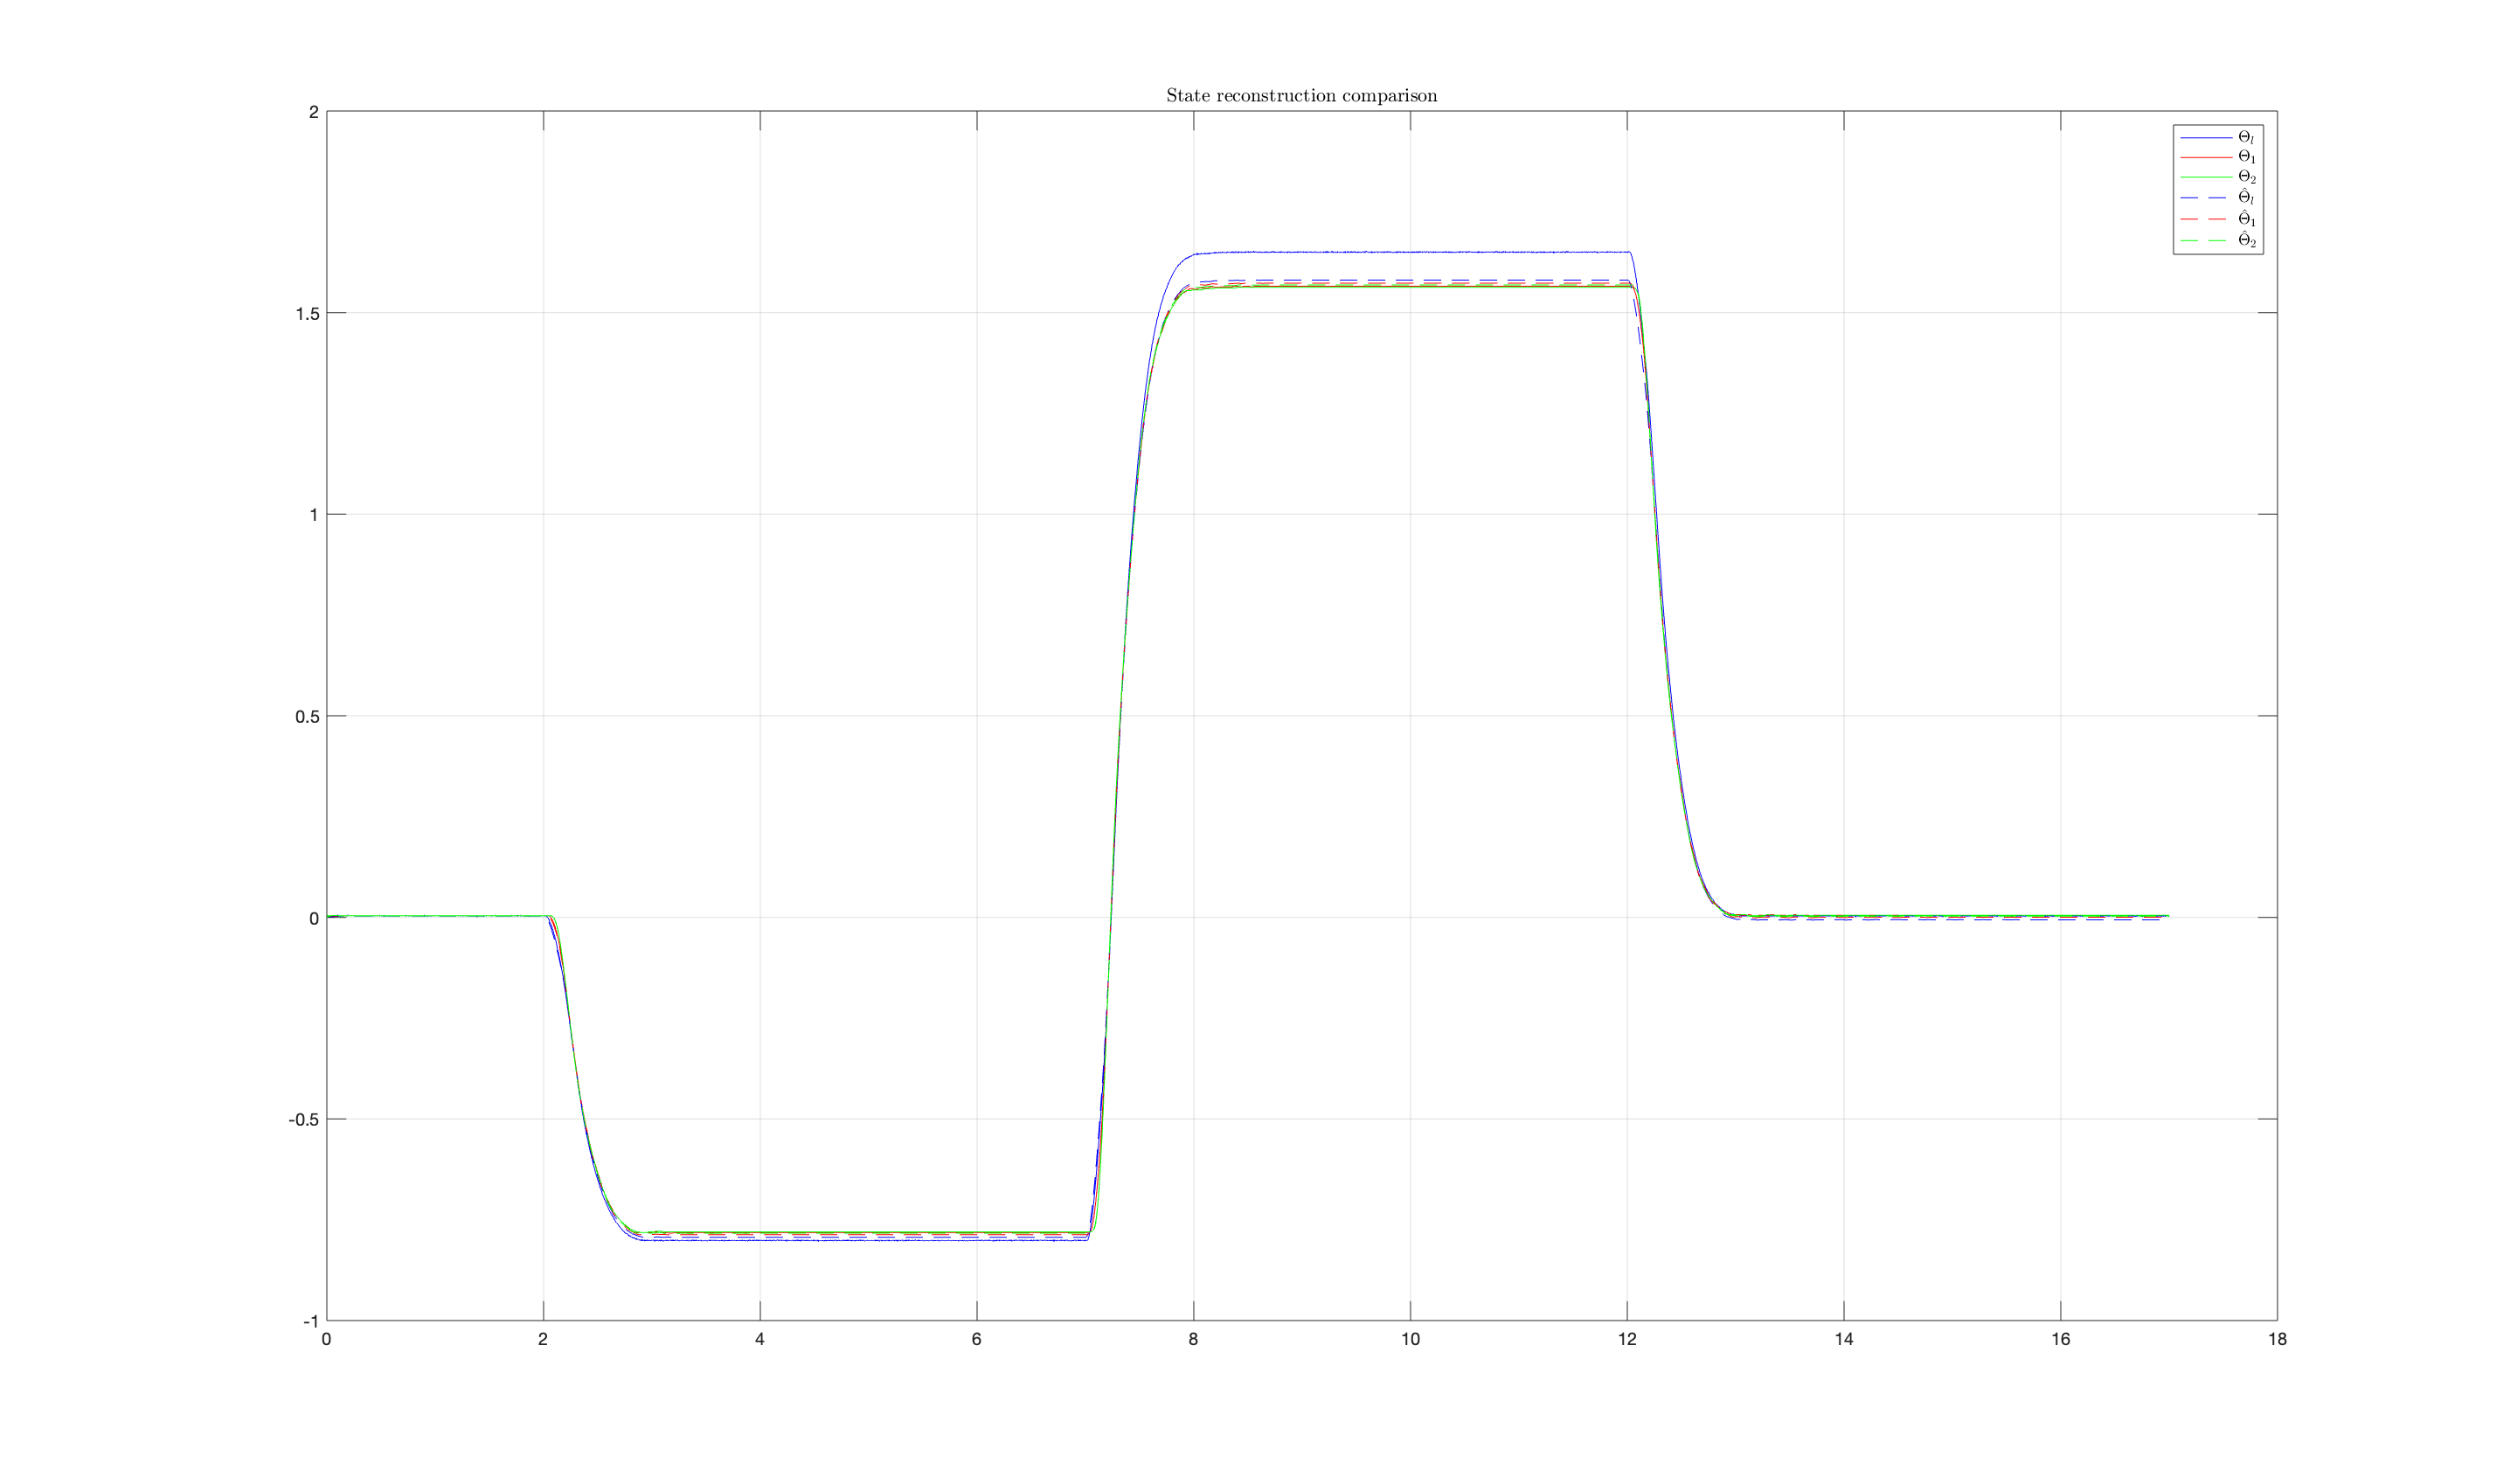
\includegraphics[width=0.8\columnwidth]{kf reconstruction 2dof.png}
	\caption{Kalman filter reconstruction compared with available measurements}
	\label{fig:kf_2dof}
\end{figure*}
In \cref{fig:kf_2dof} it is possible to see how, despite a drift in the potentiometer measurement around the second step, the reconstructed state is more related to the measurement coming from the encoders than that of the potentiometer. This happens because the noise variance of the shaft measurement is 50 times bigger than that of the encoders, making its measurement almost useless. 

\paragraph{Faulty sensor estimation}
The setup that has been used up to this point has been making use of all  the possible measurements, but after the the analysis of the reconstructed state with the kalman filter there was still a point to be analyzed. What would be the performance and the reliabilty of the system in case the encoder, that is the most rimportnat measurement, doesn't work anymore. \\
This actually happened for real during some laboratory experiment; the encoder from the second mass disconnected from the shaft and couldn't produce any results for some time. \\ 
Thus, for both systems, different state reconstructors have been developed, always based on Kalman filtering and using different combinations of the available sensors. \\
The element that change in the design of the different filters are the matrices $C$ and $D_w$. Based on the combination of sensors, different rows of the orignal $C$ and $D_w$ matrices are selected. \\
From a first analysis, all the possible setups produce an observable system, thus, applying kalman filter with the minimum number of sensor is possible in every configuration. \\
The results that are produced from these configurations can be summarized in two types. \\ 
The first can be called encoder based solution, this means that even if the measurement from the potentiometer is available, it is almost automatically discarded in favour of the encoder one. As mentioned in the previous section, this happens because the potentiometer variance is much more bigger then that one of the encoder and Riccati equations produce results that depends mostly on the lowest one. All the solutions where at least one encoder is used, produce this result and generate a state estimator with a time constant very low, allowing to push the control action to high speeds.\\
On the other hand, the solution that makes use of only the potentiometer, both in 1-d.o.f. and 2-d.o.f, generates a differnet type of filter. When only the potentiometer is used, the system matrices for the output equation (example is based on 2-d.o.f.) becomes 
\begin{equation}
	C = \begin{bmatrix}
		1 & 0 & 0 & 0 & 0 & 0
	\end{bmatrix} \
	D_w = \begin{bmatrix}
		0 & 0 & 0 & 0 & 0 & 0 & 1e-6 & 0 & 0 \\
	\end{bmatrix} 
\end{equation}
The Riccati equation that solves the filtering problem for this system produce much slower reconstructors. The time constant of the produced filter is around 0.8 seconds. Changing the parameters in the matrix $Q_x$ allows to steer a little bit the position of the poles of the estimator, but it can't move a lot the time constant of the main dynamic, mainly its damping. Indeed, the matrix $B_w$ at \ref{eqn:b_w_d_w} has been selected with those values because it was the one generating the less oscillatory response of the filter for this setup and a fast enough estimation for the other ones.\\
In order to be able to use also this setup the control action needs to be slowed down, otherwise different controllers should be tuned based on the availabilty of the sensors and logic switches could select the more appropriate controller.\\
Some tests with a switch that selects the different state reconstructors have been performed. The results are not satisfaying. In the 1-d.o.f. setup, when the controller passes from the kalman filter with all the sensors to the one with only the encoder, this isn't a problem and the system keeps following the reference, but when it starts to use the estimation derived only by the potentiometer, it diverges.This unstable behaviour is not caused by an unstable mode of the controller, but it is due to a couple of reasons. When the controller is switched the estimation changes istantaneously and so does the control action. When the two estimates are quite closed, like between the classic filter and the one with only the encoder, this sudden change results in a very small step in the voltage applied. Instead, when the estimations differ a lot, this voltage step may be too big and the saturation block limits the control action. This triggers an unstable effect, with the voltage being applied continuosly at the two saturation limits. The controller is unable to revert this, trying to apply bigger and bigger control actions to bring the state back to reference, but being limited by the saturation block. To avoid this effect, that couldn't be compensated in an easy way, the observers have been tested one at the time. \\
The results confirm partially the hyphotesis, the filters with at least one encoder for the 1-d.o.f. and at least 2 sensors for the 2-d.o.f system works well and can use the fastest controller.\\
Moreover, the 1-d.o.f. system can be controlled estimating the states from only the potentiometer measurement, but with the condition of slowing down the controller.\\
On the other hand, for the 2-d.o.f. setup it was not possible to control it using only the potentiometer, despite being able to reconstruct the states using only one of the two encoders.
In this case the reason is not completly casued by the high variance of the sensor, but it can be found in the observabilty matrix. This is full rank for all the possible combination of used measurements, but this result is obtained numerically on MATLAB. This means that even a small difference in the order of a thousands between the eigenvectores will produce a full rank matrix, so the rank analysis is not completely reliable. \\ 
To grasp this aspect, the following procedure has been followed. The rank of a matrix is the number of linearly indipendent eigenvectors.
Using SVD, it possible to extract the eigenvectors of a matrix. This method is applied to the observabilty matrix of different configurations. The numbers in the eigenvectors of the observability matrix smaller then a thousand can be neglected and then are set to zero. For the setups using only the encoders or more than one sensor the remaining vectors are clearly linearly indipendent (each couple of vectors has just 2 elements different from zero), while for the 2-d.o.f. system using only the potentiometer they appear to be more involved (there are some vectors that have up to 4 elements different from zero), hence they are not perfectly linearly indipendent.
Here it is possible to see the result of this analysis for the eigenvectors of the observality matrix of the 2-d.o.f. system with only the encoder on the last mass or with only the potentiometer. 
\begin{equation}
	e_{O_{\theta_{2}}}= \begin{bmatrix}
		0& 0 & 0 & 0 		& -0.708 & -0.706 \\
		0& 0 & 0 & 0.002 &  0.706 & -0.708 \\
		0& 0 & -0.389 & -0.921 & 0 & -0.002 \\
		0& 0 & -0.921 & -0.389 & 0 & 0 \\
		0.235 & -0.972 & 0 & 0 & 0 & 0 \\
		-0.972 & -0.235 & 0 & 0 & 0 & 0 \\
	\end{bmatrix}
\end{equation}
\begin{equation}
	e_{O_{\theta_{l}}}= \begin{bmatrix}
		0& 0 & 0 & -0.006  & 0.751 & 0.661 \\
		0& 0 & 0 & 0.096 &  -0.657 & 0.748 \\
		0& 0.002 & -0.031 & -0.995 & -0.068 & 0.068 \\
		0& -0.084 & 0.996 & -0.031 & -0.002& 0.002 \\
		-0.022 & 0.9963 & 0.084 & 0 & 0 & 0 \\
		0.999 & 0.022 & 0.002 & 0 & 0 & 0 \\
	\end{bmatrix}
\end{equation}